\chapter{Matematik}
%%
%%
\section{Polære Koordinater, Cosinus og Sinus}
%%
%%
\begin{opgave}{Idiotformlen}{1}
Brug at $\cos(\theta) $ og $\sin(\theta) $ er hhv. den hosliggende og modstående katete i en retvinklet trekant med hypotenuselængde 1 pr. deres definition. Tegn det evt. i enhedscirklen. Det giver da fra Pythagoras sætning at
\begin{align*}
\cos^2 (\theta) + \sin^2 (\theta) = 1^2 = 1 \, .
\end{align*} 
\end{opgave}
%%
%%
\begin{opgave}{Tangens}{1}
\opg Fra definitionen af tangens har man, at $\tan(\theta) = \sin(\theta)/\cos(\theta)$. Men i matematikafsnittet er det også introduceret, at $\cos(\theta)$ er givet som længden af den hosliggende katete divideret med længden af hypotenusen, og at $\sin(\theta)$ er givet som længden af den modstående katete divideret med længden af hypotenusen. For trekanten i denne opgave har man altså 
\begin{align*}
\cos(\theta) = \frac{a}{c} \quad \text{og} \quad \sin(\theta) = \frac{b}{c}  \quad \implies  \quad \tan(\theta) = \frac{\sin(\theta)}{\cos(\theta)} = \frac{\frac{b}{c}}{\frac{a}{c}} = \frac{b}{a} \, . 
\end{align*}
\opg Man finder at: $\quad \tan(\theta) = 1 \quad \implies \quad \theta =  \arctan(1) = \frac{\pi}{4} = 45\degree$.
\end{opgave}
\newpage
%%
%%
\begin{opgave}{Retvinklede trekanter}{1}
\opg Det vides, at $\cos(\theta)$ er givet som længden af den hosliggende katete divideret med længden af hypotesen. Det giver her at
\begin{align*}
\cos(\theta_{ac}) = \frac{a}{c} = \frac{5}{13} \quad \implies \quad \theta_{ac} = \arccos \left( \frac{5}{13} \right) \approx 1,176  \approx 67,38 \degree \, .
\end{align*}
\opg Ideen er her, at man for trekanten i denne opgave kan skrive $\tan(\theta_{ac}) = b/a$. Da $\theta_{ac}$ kendes fra 1) og $a$ er opgivet i opgaven, kan man nu finde $b$. Det giver
\begin{align*}
b = a \tan(\theta_{ac}) = 5 \cdot \tan \left( \arccos \left( \frac{5}{13}  \right) \right) = 12 \, .
\end{align*}
\opg Det vides, at $\sin(\theta)$ er givet som længden af den modstående katete divideret med længden af hypotesen. Det giver her at
\begin{align*}
\sin(\theta_{bc}) = \frac{a}{c} = \frac{5}{13} \quad \implies \quad \theta = \arcsin \left( \frac{5}{13} \right) \approx 0,395 \approx 22,62 \degree \, . 
\end{align*}
\end{opgave}
%%
%%
\begin{opgave}{Koordinatskift}{1}
Her bruges formlerne i \eqref{k-eq:kartesisk/polaer} fra kompendiet, altså $r = \sqrt{x^2 + y^2}$ og $\theta = \arctan\left(y/x\right)$.
\opg Man får
\begin{align*}
r = \sqrt{2^2+2^2} = \sqrt{8} \, , \quad \theta = \arctan \left( \frac{2}{2} \right) = \frac{\pi}{4} = 45 \degree \, .
\end{align*} 
\opg Man får
\begin{align*}
r = \sqrt{1^2 + (-2)^2} = \sqrt{5} \, , \quad \theta = \arctan \left( \frac{-2}{1} \right) \approx -1,107 \approx -63,43\degree \, .
\end{align*}
Det positive svar findes ved at ligge $2\pi$ radianer eller $360\degree$ til det negative resultat.
\end{opgave}
%%
%%
\begin{opgave}{Koordinatskift 2}{1}
Her bruges formlerne i \eqref{k-eq:kartesisk/polaer} fra kompendiet, altså $x = r \cos(\theta)$ og $y = r \sin(\theta)$.
\opg Man får
\begin{align*}
x = 5 \cdot \cos\left( \frac{\pi}{4} \right) = \frac{5}{\sqrt{2}} \, , \quad y = 5 \cdot \sin\left(\frac{\pi}{4}\right) = \frac{5}{\sqrt{2}} \, .
\end{align*}
\opg Man får
\begin{align*}
x = 5 \cdot \cos\left(\frac{7\pi}{4}\right) =  \frac{5}{\sqrt{2}} \, , \quad y = 5 \cdot \sin\left(\frac{7\pi}{4}\right) = - \frac{5}{\sqrt{2}} \, .
\end{align*}
\opg Man får
\begin{align*}
x = 13 \cdot \cos\left(\frac{11\pi}{6}\right) = 13 \cdot \frac{\sqrt{3}}{2} \, , \quad y = 13 \cdot \sin\left(\frac{11\pi}{6}\right) =  -13 \cdot \frac{1}{2} \, .
\end{align*}
\end{opgave}
%%
%%
\section*{Differentialregning}
%%
%%
\begin{opgave}{Hastighed og postion}{1}
	\begin{figure}[h!]
		\centering
		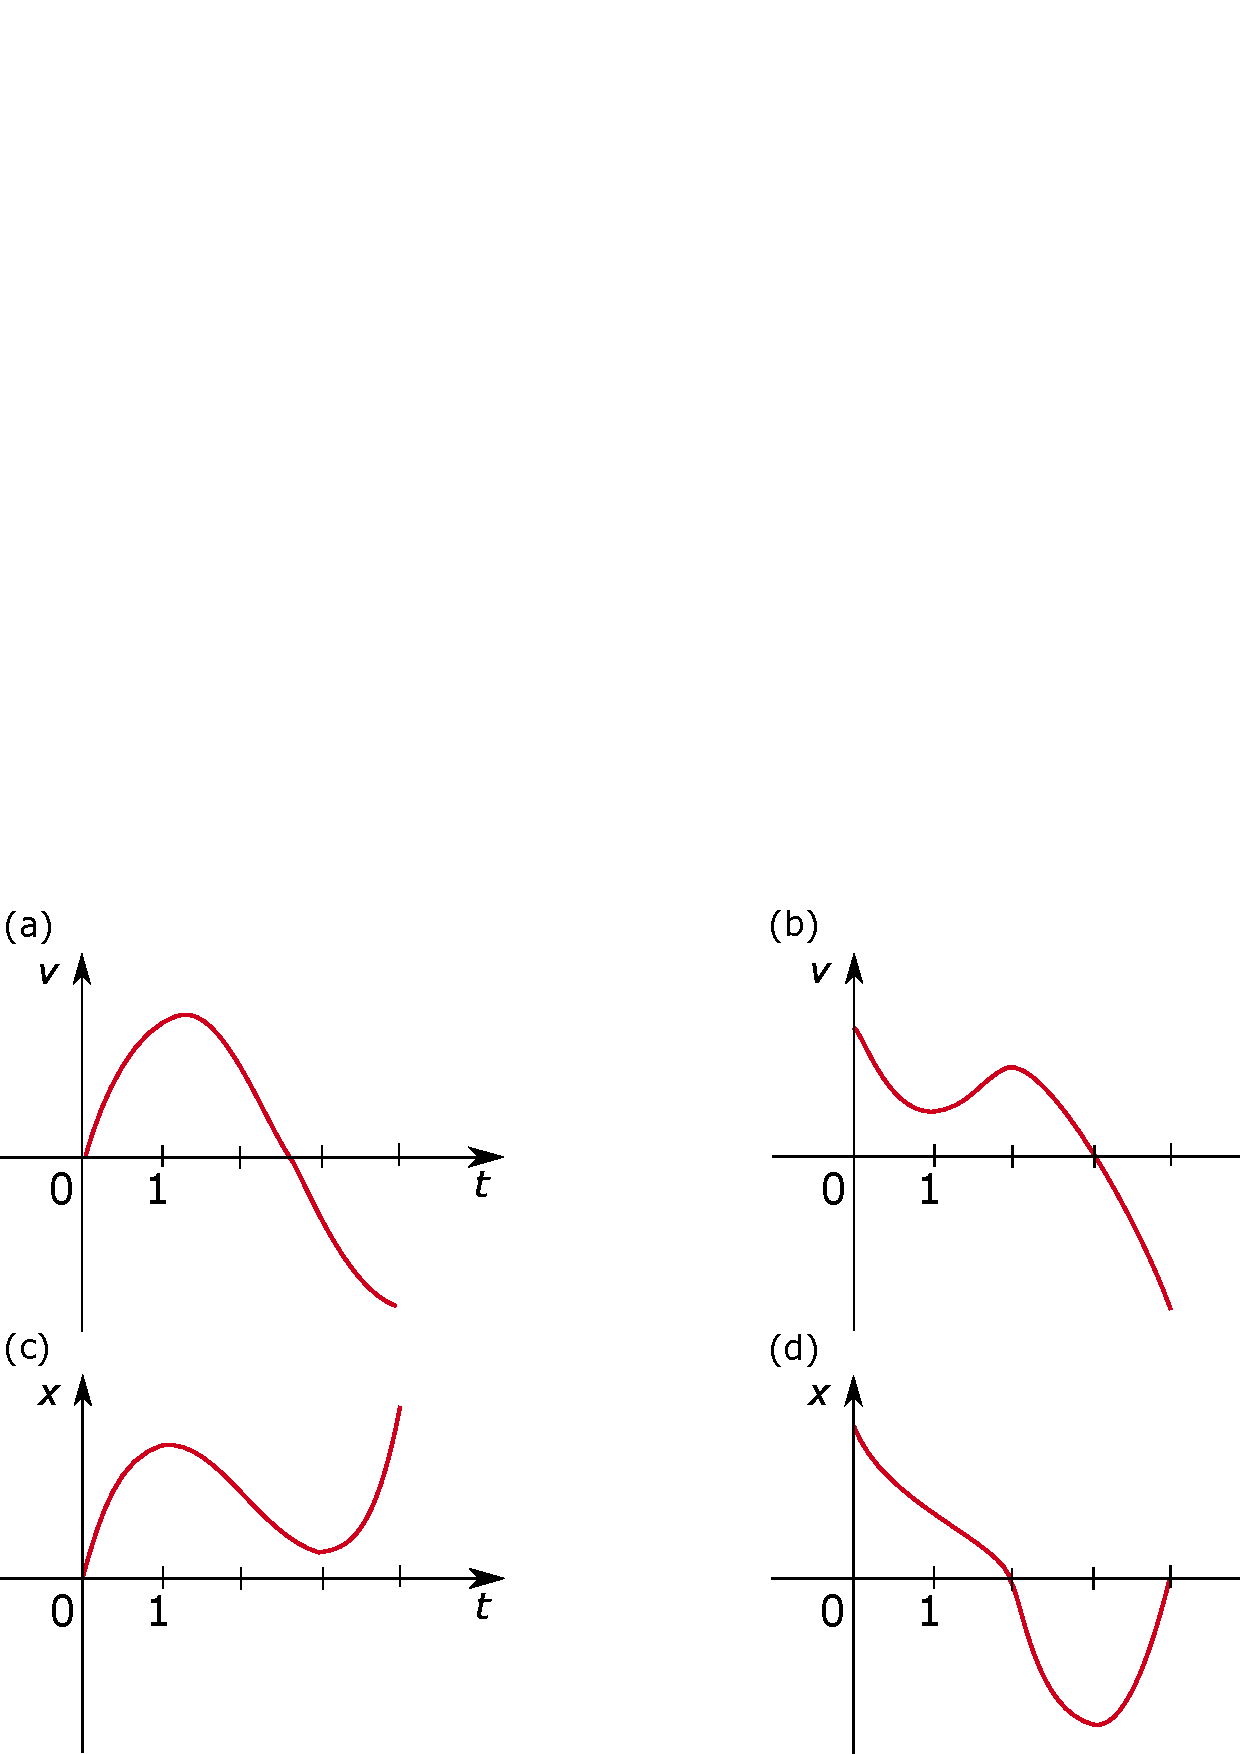
\includegraphics[width=0.47\textwidth]{matematik/vx_grafer.png}
	\end{figure}
	\opg Da graferne simpelt viser $v$ som funktion af tiden, kan man bare aflæse på figuren. For (a) har man: 
	\begin{itemize}
		\item $t= 0 \rightarrow 1,5$: sætter hastigheden op
		\item $t= 1,5 \rightarrow 4$: sætter hastigheden ned
	\end{itemize}
	For (b) har man:
	\begin{itemize}
		\item $t= 0 \rightarrow 1$: sætter hastigheden ned
		\item $t= 1 \rightarrow 2$: sætter hastigheden op
		\item $t= 2 \rightarrow 4$: sætter hastigheden ned
	\end{itemize}
	.
	\opg Her ses i stedet positionen som funktion af tiden. For at svare på hvordan hastigheden ændres med tiden, skal man derfor kigge på \emph{ændringen} i hældningen af grafen.
	For (c) har man: 
	\begin{itemize}
		\item $t= 0 \rightarrow 3$: hældningen bliver mindre/aftager $\rightarrow$ sætter hastigheden ned
		\item $t= 3 \rightarrow 4$: hældningen bliver større/vokser $\rightarrow$ sætter hastigheden op
	\end{itemize}
	For (d) har man:
	\begin{itemize}
		\item $t= 0 \rightarrow 1$: hældningen bliver meget lidt større/vokser $\rightarrow$ sætter hastigheden op
		\item $t= 1 \rightarrow 2$: hældningen bliver meget lidt mindre/aftager $\rightarrow$ sætter hastigheden ned
		\item $t= 2$: hældningen bliver meget mindre/aftager lige ved punktet 2 $\rightarrow$ sætter hastigheden hurtigt ned
		\item $t= 2 \rightarrow 4$: hældningen bliver større/vokser $\rightarrow$ sætter hastigheden op
	\end{itemize}
	.
\end{opgave}
%%
%%
\begin{opgave}{Afledede og dobbeltafledede}{1}
	\opg $f(x) = x^3$: 
	\begin{equation*}
	\dif{x}{f}=3x^2 \, , \qquad \dif[2]{x}{f}=6x \, .
	\end{equation*}
	\opg $f(x) = x^2 + 4x$:
	\begin{equation*}
	\dif{x}{f}=2x+4 \, , \qquad \dif[2]{x}{f}=2 \, .
	\end{equation*}
	\opg $f(x) = \frac{1}{x} + \frac{1}{x^2}=x^{-1}+x^{-2}$: 
	\begin{equation*}
	\dif{x}{f} = - x^{-2}-2x^{-3} \, , \qquad\dif[2]{x}{f}=2x^{-3}+6x^{-4} \, .
	\end{equation*}
	\opg $f(x) = \cos (x)$: 
	\begin{equation*}
	\dif{x}{f}= - \sin (x) \, , \qquad \dif[2]{x}{f}=-\cos (x) \, .
	\end{equation*}
	\opg $f(x) = \ln (x)$: 
	\begin{equation*}
	\dif{x}{f}= \frac{1}{x}=x^{-1} \, , \qquad \dif[2]{x}{f}=-x^{-2} \, .
	\end{equation*}
	\opg $f(x) = x\sin(x)$:
	\begin{equation*}
	\dif{x}{f} = \sin(x)+x\cos(x) \, , \qquad \dif[2]{x}{f} = 2\cos(x) - x\sin(x) \, .
	\end{equation*} 
	\opg $f(x) = \frac{1}{x}\ln(x) = x^{-1} \ln(x)$:
	\begin{equation*}
	\dif{x}{f} =  x^{-2} - x^{-2} \ln(x) = \frac{1 - \ln(x)}{x^2} \, , \qquad \dif[2]{x}{f} = -3x^{-3} + 2x^{-3}\ln(x) = \frac{2\ln(x) - 3}{x^3} \, .
	\end{equation*}
\end{opgave}
%%
%%
\begin{opgave}{Sammensatte funktioner}{1}
	Først findes $g(x)$ og så $f(g)$. Den afledede $\dif{x}{f}$ findes vha. kædereglen: $\dif{x}{f} = \dif{x}{g} \cdot \dif{g}{f}$.
	\opg $f(x) = \sin (4x)$:
	\begin{align*}
	g(x) &= 4x \, , \quad f(g)=\sin(g) \, , \quad \rightarrow \quad \dif{x}{f} = 4\cos(4x) \, .
	\end{align*}
	\opg $f(x) = \sqrt{2x}$:
	\begin{align*}
	g(x) = 2x \, , \quad f(g)=\sqrt{g} \, , \quad \rightarrow \quad \dif{x}{f} = 2\frac{1}{2\sqrt{2x}}=\frac{1}{\sqrt{2x}} \, .
	\end{align*}
	\opg $f(x) = \sqrt{4x+5}$:
	\begin{align*}
	g(x) = 4x+5 \, , \quad f(g)=\sqrt{g} \, , \quad \rightarrow \quad \dif{x}{f} = 4\frac{1}{2\sqrt{4x+5}}=\frac{2}{\sqrt{4x+5}} \, .
	\end{align*}
	\opg $f(x) = \sin(e^x)$:
	\begin{align*}
	g(x) = e^x \, , \quad f(g)=\sin(g) \, , \quad \rightarrow \quad \dif{x}{f} = e^x \cos(e^x) \, .
	\end{align*}
	\opg $f(x)=\ln(\cos(x))$:
	\begin{align*}
	g(x) = \cos(x) \, , \quad f(g) = \ln(g) \, , \quad
	\rightarrow \quad \dif{x}{f} = \left(-\sin(x)\right) \frac{1}{\cos(x)} \, .
	\end{align*}
\end{opgave}
%%
\newpage
%%
\begin{opgave}{Funktioner af flere variable - partiel differentiering}{2}
	\opg $f(x,y,z) = x+y^2+z^3$:
	\begin{align*}
	\pdif{x}{f} = 1 \, , \quad
	\pdif{y}{f} = 2y \, , \quad
	\pdif{z}{f} = 3z^2 \, .
	\end{align*}
	\opg $f(x,y,z)=xy^2+ye^{-z}$:
	\begin{align*}
	\pdif{x}{f} = y^2 \, , \quad
	\pdif{y}{f} = 2xy+e^{-z} \, , \quad
	\pdif{z}{f} = -ye^{-z} \, .
	\end{align*}
	\opg $f(x,y,z)=ze^{xyz}$:
	\begin{align*}
	\pdif{x}{f} = yz^2e^{xyz} \, , \quad
	\pdif{y}{f} = xz^2e^{xyz} \, , \quad
	\pdif{z}{f} = e^{xyz}+xyze^{xyz} \, .
	\end{align*}
	\opg $f(x,y,z) = \frac{x-y+5z}{x+y+z}$:
	\begin{align*}
	\pdif{x}{f} = \frac{2(y-2z)}{(x+y+z)^2} \, , \quad
	\pdif{y}{f} = -\frac{2(x+3z)}{(x+y+z)^2} \, , \quad
	\pdif{z}{f} = \frac{4x+6y}{(x+y+z)^2} \, .
	\end{align*}
\end{opgave}
%%
%%
\begin{opgave}{Funktioner af flere variable - total differentiering}{3}
	\opg $f(x,y,z,t) = xyz$:
	\begin{align*}
	\dif{t}{f} = yz\dif{t}{x} + xz\dif{t}{y} + xy\dif{t}{z} \, .
	\end{align*}
	\opg $f(x,y,z,t) = x+y^2+z^3$:
	\begin{align*}
	\dif{t}{f} = \dif{t}{x}+2y\dif{t}{y}+3z^2\dif{t}{z} \, .
	\end{align*}
	\opg $f(x,y,z,t) = xy^2+ye^{-z}$:
	\begin{align*}
	\dif{t}{f} = y^2\dif{t}{x}+(2xy+e^{-z})\dif{t}{y}-ye^{-z}\dif{t}{z} \, .
	\end{align*}
	\opg Da vil $\dot{x}=\dot{y}=\dot{z}=0$. Da $f(x,y,z,t)$ ikke afhænger eksplicit af $t$, får man da, at $\text{d}f/\text{d}t=0$ for 1)-3).
\end{opgave}
%%
%%
\section*{Integralregning}
%%
%%
\begin{opgave}{Ubestemte integraler}{1}
	\opg $f(x) = x^3$: 
	\begin{equation*}
	\int f(x) \d x = \frac{1}{4}x^4 +C \, .
	\end{equation*}
	\opg $f(x) = x^2 + 4x$:
	\begin{equation*}
	\int f(x) \d x = \frac{1}{3}x^3 + 2x^2 + C \, .
	\end{equation*}
	\opg $f(x) = \frac{1}{x} + \frac{1}{x^2}=x^{-1}+x^{-2}$: 
	\begin{equation*}
	\int f(x) \d x = \ln (x) -x^{-1} + C \, .
	\end{equation*}
	\opg $f(x) = \cos (x)$: 
	\begin{equation*}
	\int f(x) \d x = \sin(x)+C \, .
	\end{equation*}
	\opg $f(x) = \ln (x)$: 
	\begin{equation*}
	\int f(x) \d x = x\ln (x) -x + C \, .
	\end{equation*}
\end{opgave}
%%
%%
\begin{opgave}{Integration ved substitution}{1}
	Udregn de følgende integraler vha. integration ved substitution:
	\opg $\int e^{-4x} \d x$:
	\begin{align*}
	\int e^{-4x} \d x = -\frac{1}{4}e^{-4x} + C \, .
	\end{align*}
	\opg $\int \sqrt{3x-2} \d x$:
	\begin{align*}
	\int \sqrt{3x-2} \d x = \frac{2}{9}\cdot(3x-2)^{\frac{3}{2}} + C \, .
	\end{align*}
	\opg $\int xe^{-3x^2} \d x$:
	\begin{align*}
	\int xe^{-3x^2} \d x = -\frac{1}{6}e^{-3x^2}+C \, .
	\end{align*}
	\opg $\int \frac{x-1}{\sqrt{x+1}} \d x$:
	\begin{align*}
	\int \frac{x-1}{\sqrt{x+1}} \d x = \frac{2}{3}\sqrt{x+1}(x-5) \, .
	\end{align*}
\end{opgave}
%%
%%
\begin{opgave}{Partiel integration}{2}
	Udregn de følgende integrale vha. partiel integration:
	\opg $\int 4x\cos(2-3x)\d x$:
	\begin{align*}
	\int 4x\cos(2-3x)\d x = \frac{4}{9}\cos(2-3x)-\frac{4}{3}x\sin(2-3x) +C \, .
	\end{align*}
	\opg $\int (2+5x)e^{\frac{1}{3}x}\d x$:
	\begin{align*}
	\int (2+5x)e^{\frac{1}{3}x}\d x = (15x-39)e^{\frac{1}{3}x}+C \, .
	\end{align*}
	\opg $\int (3x+x^2)\sin (2x) \d x$:
	\begin{align*}
	\int (3x+x^2)\sin (2x) \d x = -\frac{1}{2}(3x+x^2)\cos (2x) +\frac{1}{4}\Big[ (3+2x)\sin (2x) + \cos (2x) \Big] + C \, .
	\end{align*}
\end{opgave}
%%
%%
\section*{Differentialligninger}
%%
%%
\begin{opgave}{Specialtilfælde af 1. og 2. Ordens Differentialligninger}{1}
\opg $f(t) = -7e^{3t}$ og $\dif{t}{f} = 3f(t)$.

$$\dif{t}{f} = -7 \dif{t}{} e^{3t} = -7 \cdot 3 e^{3t} = 3 \left( -7 e^{3t} \right) = 3 f(t) \, .$$
\vspace{2mm}
\opg $g(t) = \frac{2}{3}e^t + e^{-2t}$ og $\dif{t}{g} + 2g(t) = 2e^t$.

$$\dif{t}{g} = \frac{2}{3} \dif{t}{}e^t + \dif{t}{} e^{-2t} = \frac{2}{3}e^t -2e^{-2t} \quad \Rightarrow \quad \dif{t}{g} + 2g(t) = \frac{2}{3}e^t -2e^{-2t} + \frac{4}{3}e^t + 2e^{-2t} = \frac{6}{3} e^t = 2e^t \, .$$
\vspace{2mm}
\opg $h(t) = 5 \sin(3t) - 10\cos(3t)$ og $\dif[2]{t}{h} = -9h(t)$.

$$\dif{t}{h} = 3 \cdot 5 \cos(3t) + 3 \cdot 10 \sin(3t) \quad \Rightarrow \quad \dif[2]{t}{h} = (-9) \cdot 5 \cos(3t) + 9 \cdot 10 \sin(3t) = -9 h(t) \, .$$
\vspace{2mm}
\opg $k(t) = 13 \cos \left( 8t + 45 \right)$ og $\dif[2]{t}{k} = -64 k(t)$.

$$\dif{t}{k} = (-8) \cdot 13 \cos \left( 8t + 45 \right) \quad \Rightarrow \quad \dif[2]{t}{k} = (-64) \cdot 13 \cos \left( 8t + 45 \right) = -64 k(t) \, .$$
\vspace{2mm}
\end{opgave}
%%
%%
\begin{opgave}{Generelle 1. Ordens Differentialligninger}{2}
\opg $h(x) = 1/ \left( x+A \right)$ og $\dif{x}{h} = -h(x)^2$.

$$\dif{x}{f} = \dif{x}{}\left( x+A \right)^{-1} = - \left( x+A \right)^{-2} \dif{x}{}\left( x+A \right) = - \frac{1}{\left( x + A \right)^2} = -h(x)^2 \, .$$
\vspace{2mm}
\opg $k(x) = \left( c-x^2 \right)^{-1/2}$ og $\dif{x}{k} = x k(x)^3$.

$$\dif{x}{k} = - \frac{1}{2} \left( c-x^2 \right)^{-3/2}  \dif{x}{}\left( c-x^2 \right) = x \left( c-x^2 \right)^{-3/2} = x k(x)^3 \, .$$
\vspace{2mm}
\opg $g(x) = \left( \ln (x) + C \right)/x$ og $x^2 \dif{x}{g} + x g(x) = 1$.

\begin{align*}
	\dif{x}{g} &= \left[ \dif{x}{}\left( \ln x + C \right) \right] \frac{1}{x} + \left( \ln x + C \right)  \left[ \dif{x}{}\frac{1}{x} \right]  = \frac{1}{x^2} - \frac{\ln x + C}{x^2}  \\ &\Rightarrow x^2 \dif{x}{g} + xg(x) = 1 - \left( \ln (x) + C \right) + \left( \ln (x) + C \right) = 1 \, .
\end{align*}
\vspace{2mm}
\opg $f(x) = \left( 1+ce^x \right)/\left( 1-ce^x \right)$ og $\dif{x}{f} = \frac{1}{2} \left( f(x)^2 -1 \right)$.

\begin{align*}
\dif{x}{f} &= \left[ \dif{x}{}\left( 1+c^x \right) \right] \frac{1}{1-ce^x} + \left( 1+ce^x \right) \left[ \dif{x}{}\frac{1}{1-ce^x} \right] = \frac{ce^x}{1-ce^x} +  \frac{\left( 1+ce^x \right) \left( -1 \right) \left( -ce^x \right)}{\left( 1-ce^x \right)^2} \\
&= ce^x \left[ \frac{1}{1-ce^x} + \frac{1+ce^x}{\left( 1-ce^x \right)^2} \right] = ce^x \frac{1-ce^x + 1+ce^x}{\left( 1-ce^x \right)^2} = \frac{2ce^x}{\left( 1-ce^x \right)^2} \, .
\end{align*}

\begin{align*}
	f(x)^2 - 1  &=  \frac{\left( 1+ce^x \right)^2}{\left( 1-ce^x \right)^2} - \frac{(1-ce^x)^2}{\left( 1-ce^x \right)^2} = \frac{\left( 1+ce^x \right)^2 - \left( 1-ce^x \right)^2}{\left( 1-ce^x \right)^2} = \frac{4ce^x}{\left( 1-ce^x \right)^2} = 2 \dif{x}{f} \, .
\end{align*}
\end{opgave}
%%
%%
\begin{opgave}{Hvornår er det en løsning?}{3}
\opg Find $k$ så $f(y) = \cos(ky)$ løser $4 \dif[2]{y}{f} = -25f(y)$.

$$\dif{y}{f} = -k\sin(ky) \quad \Rightarrow \quad \dif[2]{y}{f} = -k^2 \cos(ky) = -k^2 f(y) \, .$$

\vspace{2mm}

Så sætter man ind:

$$4 \dif[2]{y}{f} = -25f(y) \quad \Rightarrow \quad -4k^2 f(y) = -25f(y) \quad \Rightarrow \quad k^2 = \frac{25}{4} \quad \Rightarrow \quad k = \pm \frac{5}{2} \, .$$
\vspace{2mm}
\opg For de fundne $k$ fra 1), vis at $g(y) = A\sin(ky) + B\cos(ky)$ løser $4 \dif[2]{y}{g} = -25g(y)$.

$$\dif{y}{g} = kA\cos(ky) - kB\sin(ky) \quad \Rightarrow \quad \dif[2]{y}{g} = -k^2 A \sin(ky) - k^2 B \cos(ky) = -k^2g(y) \, .$$

\vspace{2mm}

Det giver:

$$-4k^2 g(y) = -25g(y) \, .$$

\vspace{2mm}

Som er opfyldt for $k = \pm \frac{5}{2}$.\\
\opg Find $r$ så $h(y) = e^{ry}$ løser $2 \dif[2]{y}{h} + \dif{y}{h} - h(y) = 0$.

$$\dif{y}{h} = re^{ry} = rh(y) \quad \Rightarrow \quad \dif[2]{y}{h} = r^2 e^{ry} = r^2 h(y) \, .$$

\vspace{2mm}

Så sætter man ind:

$$2 \dif[2]{y}{h} + \dif{y}{h} - h(y) = 0 \quad \Rightarrow \quad 2r^2h(y) + rh(y) -h(y) = 0 \quad \Rightarrow \quad 2r^2+r-1=0 \, .$$
\vspace{2mm}

Løses andengradsligningen får man:

$$r_1 = \frac{1}{2} \quad \text{og} \quad r_2 = -1 \, .$$ 
\vspace{2mm}
\opg For de fundne $r_1,r_2$ i 3), vis at $k(y) = ae^{r_1y} + be^{r_2y}$ løser $2 \dif[2]{y}{k} + \dif{y}{k} - k(y) = 0$.

$$\dif{y}{k} = ar_1e^{r_1y} + br_2e^{r_2y} \quad \Rightarrow \quad \dif[2]{y}{k} = ar_1^2e^{r_1y} + br_2^2e^{r_2y} \, .$$ 
\vspace{2mm}

Så sætter man ind:
\begin{align*}
2 \dif[2]{y}{k} + \dif{y}{k} - k(y) &= 2 \left( ar_1^2e^{r_1y} + br_2^2e^{r_2y}  \right) + \left( ar_1e^{r_1y} + br_2e^{r_2y} \right) - \left( ae^{r_1y} + be^{r_2y} \right)\\
&= \left( 2ar_1^2 + ar_1 - a \right)e^{r_1y} + \left( 2br_2^2 + br_2 - b \right)e^{r_2y} \\
 &= a\left( 2r_1^2 + r_1 - 1 \right)e^{r_1y} + b\left( 2r_2^2 + r_2 -  \right)e^{r_2y} = 0 \cdot e^{r_1y} + 0 \cdot e^{r_2y} = 0 \, .
\end{align*}
\end{opgave}
%%
%%
\section*{Taylorapproksimationer}
%%
%%
\begin{opgave}{Taylorpolynomier for simple funktioner}{2}
	\opg $f(x)=\cos(x)$:
	\begin{align*}
	T_0(x) &= \cos(a) \, , \\
	T_1(x) &= \cos(a) - \sin(a)(x-a) \, , \\
	T_2(x) &= \cos(a) - \sin(a)(x-a) - \frac{1}{2}\cos(a)(x-a)^2 \, .
	\end{align*}
	\opg $f(x) = \sin(x)$:
	\begin{align*}
	T_0(x) &= \sin(a) \, , \\
	T_1(x) &= \sin(a) + \cos(a)(x-a) \, ,  \\
	T_2(x) &= \sin(a) + \cos(a)(x-a) -\frac{1}{2}\sin(a)(x-a)^2 \, .
	\end{align*}
	\opg $f(x) = e^x$:
	\begin{align*}
	T_0(x) &= e^a \, , \\
	T_1(x) &= e^a + e^a(x-a) \, , \\
	T_2(x) &= e^a + e^a(x-a) + \frac{1}{2}e^a(x-a)^2 \, .
	\end{align*}
\end{opgave}
%%
%%
\begin{opgave}{Jordens form}{2}
	I første omgang differentieres funktionen to gange vha. kædereglen
	\begin{align*}
	\dif{x}{f(x)} &= \frac{1}{2}\left[R^2 - x^2\right]^{-1/2}(-2x) = \frac{-x}{\sqrt{R^2 - x^2}} \, , \\
	\dif[2]{x}{f(x)} &= \dif{x}{}\left(\frac{-x}{\sqrt{R^2 - x^2}}\right) = -\frac{1}{2}(-x)\left[R^2 - x^2\right]^{-3/2}(-2x) - \left[R^2 - x^2\right]^{-1/2} \\
	&= \frac{-x^2}{(R^2 - x^2)^{3/2}} - \frac{1}{\sqrt{R^2 - x^2}} \, .
	\end{align*}
	Evalueres disse differentialer i $x = 0$ fås
	\begin{align*}
	\left.\dif{x}{f(x)}\right|_{x=0} &= \left[\frac{-x}{\sqrt{R^2 - x^2}}\right]_{x=0} = \frac{-0}{\sqrt{R^2 - 0^2}} = 0 \, , \\
	\left.\dif[2]{x}{f(x)}\right|_{x=0} &= \left[\frac{-x^2}{(R^2 - x^2)^{3/2}} - \frac{1}{\sqrt{R^2 - x^2}}\right]_{x=0} = \frac{-0^2}{(R^2 - 0^2)^{3/2}} - \frac{1}{\sqrt{R^2 - 0^2}} \\
	&= 0 - \frac{1}{R} = -\frac{1}{R} \, .
	\end{align*}
	\opg Indsættes det i ligning \eqref{k-Taylor_pol} fra kompendiet fås
	\begin{align*}
	T_2(x) = f(0) + x\left.\dif{x}{f(x)}\right|_{x=0} + \frac{1}{2}x^2\left.\dif[2]{x}{f(x)}\right|_{x=0} = R + 0 - \frac{1}{R}x^2 = R-\frac{1}{2R}x^2 \, .
	\end{align*}
	hvilket er Taylorpolynomiet til 2. orden. Til nulte og første orden er det
	\begin{align*}
	T_0(x) = R \, , \qquad T_1(x) = R + 0 = R \, .
	\end{align*}
	\opg Da $T_0(x) = T_1(x)$ betragtes de herfra sammen.
	\begin{itemize}
		\item $T_1$ er en vandret linje for alle værdier af $x$.
		\item $T_2(x)$ er en parabel, hvor "benene" $\, ,$ vender nedad, grundet fortegnet på 2.ordensleddet.
	\end{itemize}
	.
	\opg Se figur \ref{fig:JordensForm}.
	\opg Der er tale om:
	\begin{itemize}
		\item Til 0. og 1. orden får man et plan.
		\item 	Til 2. får man en elliptisk paraboloid, dvs. den figur der fremkommer ved at dreje en parabel \SI{180}{\degree} rundt om $y$-aksen. Af denne figur er taget de positive værdier og spejlet i $x$-aksen. Denne forklaring giver ikke super meget mening, hvorfor det er bedre bare at tænke det som et øje.
	\end{itemize}
	.
	\opg På baggrund af dette er det acceptable approksimationer at se Jorden som enten flad eller et gigantisks øje. Som figuren dog viser er det begrænset, i hvor stort et område disse approksimationer er valide.
\end{opgave}
\begin{figure}[h!]
	\centering
	\includegraphics[trim=3.9cm 9.4cm 4cm 9.4cm,width=0.6\columnwidth]{matematik/fig/JordensForm.pdf}
	\caption{Plot af $f(x),g(x)$, samt approksimationer af disse.} \label{fig:JordensForm}
\end{figure}
%%
%%
\section{Komplekse tal}
%%
%%
\begin{opgave}{Den komplekse plan}{1}
Tallene er indtegnet på følgende billede.
\begin{figure}[h!]
	\centering
	\includegraphics[scale=0.6]{matematik/fig/komplekse_tal_i_plan_opg.png}
\end{figure}
\end{opgave}
%%
%%
\begin{opgave}{Regning med komplekse tal}{1}
Her bruges $z_1 = 3+2i, \, \, z_2 = -6+i, \, \, z_3 = 1-5i, \, \, z_4 = -4+3i$.\\
\opg Man får $z_1+z_2 = -3+3i$ og $z_3+z_4 = -3-2i$.
\opg Man får $z_1-z_2 = 9+i$ og  $z_3-z_4 = 5-8i$.
\opg Man får $z_1z_2 = -20-9i$ og $z_3z_4 = 11+23i$.
\opg Man får $z_1/z_2 = -(16/37) - (15/37)i$ og $z_3/z_4 = -(19/25)+(17/25)i$.
\opg Man får $\abs{z_1} = \sqrt{13}$ og $\abs{z_2} = \sqrt{37}$. Endeligt får man, at $\abs{z_3z_4} = \abs{z_3} \abs{z_4} = 5 \cdot \sqrt{26}$.
\end{opgave}
%%
%%
\begin{opgave}{Regneregler for modulus og normkvadratet}{2}
\opg Regnereglerne tages en af gangen. Lad $z_1 = a+bi$ og $z_2 = c+di$.\\ \\
Først \eqref{k-modulus_regneregler1}:
\begin{align*}
\abs{z_1} = \abs{a+bi} = \sqrt{a^2+b^2} = \sqrt{a^2+\left(-b\right)^2} = \abs{a-bi} = \abs{z_1^*} \, .
\end{align*}
Så \eqref{k-modulus_regneregler2}:
\begin{align*}
\abs{z_1z_2} &= \abs{\left(ac-bd\right) + \left(ad+bc\right)i} = \sqrt{\left(ac-bd\right)^2 + \left(ad+bc\right)^2} = \sqrt{\left(ac\right)^2 + \left(bc\right)^2 + \left(ad\right)^2 + \left(bc\right)^2} \\
&= \sqrt{\left(a^2+b^2\right) \cdot \left(c^2+d^2\right)} = \sqrt{a^2+b^2} \cdot\sqrt{c^2+d^2} = \abs{z_1}\abs{z_2} \, .  
\end{align*}
Endeligt \eqref{k-modulus_regneregler3}. Her bemærker man først at
\begin{align*}
\abs{z_1^n} = \abs{\left(z_1^{n-1}\right)z_1} = \abs{z_1^{n-1}}\abs{z_1} \, , 
\end{align*}
hvor \eqref{k-modulus_regneregler2} er brugt i  den anden lighed. Man kan da lave samme trick for $z_1^{n-1}$
\begin{align*}
\abs{z_1^{n-1}} = \abs{\left(z_1^{n-2}\right)z_1} = \abs{z_1^{n-2}}\abs{z_1} \, ,
\end{align*}  
hvilket viser at
\begin{align*}
\abs{z_1^n} = \abs{z_1^{n-1}}\abs{z_1} = \abs{z_1^{n-2}}\abs{z_1}\abs{z_1} \, .
\end{align*}
Ideen er da blot at fortsætte på samme vis, hvilket giver det ønskede resultat. Streng taget burde dette laves som et \emph{induktionsbevis}, hvis det skulle være helt matematisk korrekt, men metoden her er mere intuitiv og illustrerer ideen i beviset.
\opg Her vises formel \eqref{k-normkvadrat2}. Lad $z=a+bi$.
\begin{align*}
\abs{z}^2 = \left(\sqrt{a^2+b^2}\right)^2 = a^2+b^2 = \left(a+bi\right)\left(a-bi\right) = zz^* \, .
\end{align*}
\end{opgave}
%%
%%
\begin{opgave}{Eulers formel og komplekse tal på polær form}{3}
\opg De komplekse tal for de forskellige værdier af $x$ bliver:
\begin{align*}
e^{i \cdot 0} = 1 \, , \qquad e^{i \cdot \frac{\pi}{2}} = i \, , \qquad e^{i \cdot \pi} = -1 \, , \qquad e^{i \cdot \frac{3\pi}{2}} = -i \, .
\end{align*}
Altså bevæger $e^{ix}$ sig rundt mod uret i den komplekse plan, når $x$ vokser.
\opg Fra Eulers formel har man at
\begin{align*}
\abs{e^{ix}} = \abs{\cos(x) + i \sin(x)} = \sqrt{\cos^2(x) + \sin^2(x)} = \sqrt{1} = 1 \, .
\end{align*}
Altså  er modulus af $e^{ix}$ konstant og ændres derfor ikke, når man ændrer $x$.
\opg Her kan man bruge de samme $x$ som fra 1). Det giver
\begin{align*}
e^{-i \cdot 0} = 1 \, , \qquad e^{-i \cdot \frac{\pi}{2}} = -i \, , \qquad e^{-i \cdot \pi} = -1 \, , \qquad e^{-i \cdot \frac{3\pi}{2}} = i \, .
\end{align*}
Altså bevæger $e^{-ix}$ sig rundt med uret i den komplekse plan, når $x$ vokser.
\opg Fra Eulers formel har man at
\begin{align*}
\abs{e^{-ix}} = \abs{\cos(-x) + i \sin(-x)} = \abs{\cos(x) - i \sin(x)} = \sqrt{\cos^2(x) + \left(-\sin(x)\right)^2} = \sqrt{1} = 1 \, ,
\end{align*}
hvor det er benyttet at $\cos(-x) = \cos(x)$ og at $\sin(-x) = -\sin(x)$. Dette skyldes at cosinus er en lige funktion, mens sinus er en ulige funktion. Altså  er modulus af $e^{-ix}$ konstant og ændres derfor ikke, når man ændrer $x$.
\opg Først bemærkes det, hvis man tegner $z=a+bi$ i den komplekse plan, at man vha. $z$'s modulus, $\abs{z}$, og argument, $\theta$, kan skrive $a$ og $b$ som følger
\begin{align*}
a = \abs{z} \cos(\theta)  \qquad \text{og} \qquad b = \abs{z}\sin(\theta) \, .
\end{align*}
Bruger man da Eulers formel, får man at
\begin{align*}
z = a+bi = \abs{z}\cos(\theta)+i\abs{z}\sin(\theta) = \abs{z}\left(\cos(\theta)+i\sin(\theta)\right) = \abs{z}e^{i\theta} \, .
\end{align*}
\end{opgave}
%%
%%
\begin{opgave}{Komplekse ligninger}{2}
\opg Der løses for $z$ som i en normal ligning.
\begin{align*}
\frac{z-2}{z+1} = 3i \quad &\implies \quad z-2 = 3i\left(z+1\right) = 3i \cdot z + 3i \quad \implies \quad z - 3i \cdot z = 2 + 3i \\
&\implies z  \left(1-3i\right) = 2+3i \quad \implies \quad z = \frac{2+3i}{1-3i} = -\frac{7}{10} +  \frac{9}{10}i \, .
\end{align*}
\opg Her bruges en anden metode end i 1), for at vise at komplekse ligninger kan løses på forskellige måder. Ideen er at skrive $z=a+bi$, hvor man ikke kender $a$ og $b$ endnu. Dette indsættes i venstresiden af ligningen, og der reduceres
\begin{align*}
z + 3z^* = a+bi + 3(a-bi) = 4a -2bi \, .
\end{align*}
Sammenligner man da med højresiden af ligningen, $5-6i$, giver dette to normale ligninger, da realdelen af venstresiden må være lig med realdelen af højresiden og ligeledes for imaginærdelene. Altså får man ligningerne:
\begin{align*}
4a = 5 \qquad \text{og} \qquad -2b = -6 \, .
\end{align*}
Disse ligninger har løsningerne $a=5/4$ og $b=3$, og løsningen af den komplekse ligning er da
\begin{align*}
z = \frac{5}{4} + 3i \, .
\end{align*}
\end{opgave}
%%
%%
\section*{Vektorer}
%%
%%
\begin{opgave}{Længden af en vektor}{1}
	\begin{align*}
	\abs{\v{v_1}} = \sqrt{1^2+2^2+3^2} = \sqrt{14} \, , \\
	\abs{\v{v_2}} = \sqrt{(-4)^2+5^2+0^2} = \sqrt{41} \, .
	\end{align*}
\end{opgave}
%%
%%
\begin{opgave}{Addition, subtraktion og skalarmultiplikation med vektorer}{1}
	\opg $\v{v_1}+\v{v_2}$:
	\begin{align*}
	\begin{bmatrix} 1 \\ 2 \\ 3 \end{bmatrix} + \begin{bmatrix} -4 \\ 5 \\ 0 \end{bmatrix} = \begin{bmatrix} 1-4 \\ 2+5 \\ 3+0 \end{bmatrix} = \begin{bmatrix} -3 \\ 7 \\ 3 \end{bmatrix} \, .
	\end{align*}
	\opg $\v{v_1}-\v{v_2}$:
	\begin{align*}
	\begin{bmatrix} 1 \\ 2 \\ 3 \end{bmatrix} - \begin{bmatrix} -4 \\ 5 \\ 0 \end{bmatrix} = \begin{bmatrix} 1+4 \\ 2-5 \\ 3-0 \end{bmatrix} = \begin{bmatrix} 5 \\ -3 \\ 3 \end{bmatrix} \, .
	\end{align*}
	\opg $5\cdot\v{v_1}$ og $5\cdot\v{v_2}$:
	\begin{align*}
	5 \cdot \begin{bmatrix} 1 \\ 2 \\ 3 \end{bmatrix} &= \begin{bmatrix} 5\cdot 1 \\ 5\cdot 2 \\ 5\cdot 3 \end{bmatrix} = \begin{bmatrix} 5 \\ 10 \\ 15 \end{bmatrix} \, , \\
	5 \cdot \begin{bmatrix} -4 \\ 5 \\ 0 \end{bmatrix} &= \begin{bmatrix} -5\cdot 4 \\ 5\cdot 5 \\ 5\cdot 0 \end{bmatrix} = \begin{bmatrix} -20 \\ 25 \\ 0 \end{bmatrix} \, .
	\end{align*}
	\opg $5\cdot(\v{v_1}\pm\v{v_2})$ og $5\cdot\v{v_1}\pm 5\cdot\v{v_2}$:
	\begin{align*}
	5\cdot(\v{v_1} + \v{v_2}) &= 5\cdot \begin{bmatrix} 1-4 \\ 2+5 \\ 3+0 \end{bmatrix} = 5 \cdot \begin{bmatrix} -3 \\ 7 \\ 3 \end{bmatrix} = \begin{bmatrix} -15 \\ 35 \\ 15 \end{bmatrix} \, , \\
	5\cdot(\v{v_1}-\v{v_2}) &= 5\cdot \begin{bmatrix} 1+4 \\ 2-5 \\ 3-0 \end{bmatrix} = 5 \cdot \begin{bmatrix} 5 \\ -3 \\ 3+0 \end{bmatrix} = \begin{bmatrix} 25 \\ -15 \\ 15 \end{bmatrix} \, , \\
	5\cdot\v{v_1} + 5\cdot\v{v_2} &= 5\cdot \begin{bmatrix} 1 \\ 2 \\ 3 \end{bmatrix} + 5\cdot \begin{bmatrix} -4 \\\ 5 \\ 0 \end{bmatrix} = \begin{bmatrix} 5 \\ 10 \\ 15 \end{bmatrix} + \begin{bmatrix} -20 \\ 25 \\ 0 \end{bmatrix} = \begin{bmatrix} -15 \\ 35 \\ 15 \end{bmatrix} \, , \\
	5\cdot\v{v_1} - 5\cdot\v{v_2} &= 5\cdot \begin{bmatrix} 1 \\ 2 \\ 3 \end{bmatrix} - 5\cdot \begin{bmatrix} -4 \\\ 5 \\ 0 \end{bmatrix} = \begin{bmatrix} 5 \\ 10 \\ 15 \end{bmatrix} - \begin{bmatrix} -20 \\ 25 \\ 0 \end{bmatrix} = \begin{bmatrix} 25 \\ -15 \\ 15 \end{bmatrix} \, .
	\end{align*}
	Dette resultat betyder, at man ved skalarmultiplikation kan gange ind i parenteser, ligesom man kender det for normale tal. Altså
	\begin{align*}
	a\cdot \left( \v{v}_1 \pm \v{v}_2 \right) = a \cdot \v{v}_1 \pm a \cdot \v{v}_2 \, , \qquad \text{ligesom} \qquad a\left(b+c\right) = ab + ac \, .
	\end{align*} 
\end{opgave}
%%
%%
\begin{opgave}{Skalarproduktet}{2}
	\opg $\v{v_1}\cdot \v{v_2}$:
	\begin{align*}
	\v{v_1}\cdot \v{v_2} = \v{v_2}\cdot \v{v_1} = -4+10 = 6 \, .
	\end{align*}
	\opg Der tjekkes kun for $\v{v}_1$. Man får
	\begin{align*}
	\abs{\v{v}_1} = \sqrt{14} \, , \qquad \sqrt{\v{v}_1 \cdot \v{v}_1} = \sqrt{1^2+2^2+3^2} = \abs{\v{v}_1} \, .
	\end{align*}
	\opg
	\begin{align*}
	\theta = \arccos \left( \frac{\v{v_1}\cdot \v{v_2}}{\abs{\v{v_1}}\cdot\abs{\v{v_2}}} \right)  = \arccos \left({\frac{6}{\sqrt{14}\cdot\sqrt{41}}}\right) \approx 1,318 \approx \ang{75,5} \, .
	\end{align*}
\end{opgave}
%%
%%
\begin{opgave}{Krydsproduktet}{2}
	\opg $\v{v_1} \times \v{v_2} \, \,  \text{og} \, \,  \v{v_2}\times \v{v_1}$:
	\begin{align*}
	\v{v_1} \times \v{v_2} &=  \begin{bmatrix} -15 \\ -12 \\ 13 \end{bmatrix} \, , \\
	\v{v_2} \times \v{v_1} &= \begin{bmatrix} 15 \\ 12 \\ -13 \end{bmatrix} \, .
	\end{align*}
	Altså har man at $	\v{v_1} \times \v{v_2} = - \v{v_2} \times \v{v_1}$.
	\opg $\abs{\v{v_1} \times \v{v_2}}$:
	\begin{align*}
	\abs{\v{v_1} \times \v{v_2}} = \sqrt{(-15)^2+(-12)^2+13^2} = \sqrt{538} \, .
	\end{align*}
	\opg 
	\begin{align*}
	\theta = \arcsin\left(\frac{\abs{\v{v_1} \times \v{v_2}}}{\abs{\v{v_1}}\abs{\v{v_2}}}\right) = \arcsin\left( \frac{\sqrt{538}}{\sqrt{14}\cdot\sqrt{41}} \right) \approx 1,318 \approx \ang{75,5} \, . 
	\end{align*}
\end{opgave}
%%
%%
\begin{opgave}{Regning med enhedsvektorer}{2}
	\opg
	\begin{align*}
	\v{v_1} = v_{x1}\xhat+v_{y1}\yhat+v_{z1}\zhat \, , \qquad 
	\v{v_2} = v_{x2}\xhat+v_{y2}\yhat+v_{z2}\zhat \, .
	\end{align*}
	\opg Det passer.
	\opg
	\begin{align*}
	\xhat\cdot\xhat = 1 \, , \quad
	\xhat\cdot\yhat = 0 \, , \quad
	\xhat\cdot\zhat = 0 \, , \quad
	\yhat\cdot\yhat = 1 \, , \quad
	\yhat\cdot\zhat = 0 \, , \quad
	\zhat\cdot\zhat = 1 \, .
	\end{align*}
	Resten regnes på samme måde.
	\opg Det giver det samme.
	\opg Her skrives nulvektoren $\v{0}$, altså vektoren hvor alle indgange er nul.
	\begin{align*}
	\xhat\times\xhat = \v{0} \, , \quad 
	\xhat\times\yhat = \zhat \, , \quad
	\xhat\times\zhat = -\yhat \, , \quad
	\yhat\times\yhat = \v{0} \, , \quad
	\yhat\times\zhat = \xhat \, , \quad
	\zhat\times\zhat = \v{0} \, .
	\end{align*}
	Resten regnes på samme måde.
	\opg Det giver det samme.
\end{opgave}